Para encontrar un algoritmo de Programación Dinámica que lo resuelva, primero hemos de plantear el problema como una secuencia de decisiones que verifique el
principio de óptimo. De aquí seremos capaces de deducir una expresión recursiva de la solución. Por último habrá que encontrar una estructura de datos adecuada
que permita la reutilización de los cálculos de la ecuación en recurrencia, consiguiendo una complejidad mejor que la del algoritmo puramente recursivo.

Siendo M la capacidad de la mochila y disponiendo de n elementos, llamaremos V(i,p) al valor máximo de la mochila con capacidad p cuando consideramos i
objetos, con 0 $\leq$ p $\leq$ M y 1 $\leq$ i $\leq$ n. La solución viene dada por el valor de V(n,M). Denominaremos d$_{ 1}$ , d$_{ 2}$ , ..., d$_{ n}$ a la secuencia de decisiones que conducen a obtener V(n,M), donde cada d$_{ i}$ podrá tomar uno de los valores 1 ó 0, dependiendo si se introduce o no el i-ésimo elemento. Podemos tener por tanto dos situaciones distintas:

\begin{itemize}
	\item Que d$_{ n}$ = 1. La subsecuencia de decisiones d$_{ 1}$ , d$_{ 2}$ , ..., d$_{ n-1}$ ha de ser también
	óptima para el problema V(n–1,M–p$_{ n}$ ), ya que si no lo fuera y existiera otra subsecuencia e$_{ 1}$ , e$_{ 2}$ , ..., e$_{n-1}$ óptima, la secuencia e$_{ 1}$ , e$_{ 2}$ , ..., e$_{n-1}$ , d$_{n}$ también sería óptima para el problema V(n,M) lo que contradice la hipótesis.
	\item Que d$_{ n}$ = 0. Entonces la subsecuencia decisiones d$_{ 1}$ , d$_{ 2}$ , ..., d$_{ n-1}$ ha de ser también
	óptima para el problema V(n–1,M).
\end{itemize}

Podemos aplicar por tanto el principio de óptimo para formular la relación en recurrencia. Teniendo en cuenta que en la mochila no puede introducirse una fracción del elemento sino que el elemento i se introduce o no se introduce, en una situación cualquiera V(i,p) tomará el valor mayor entre V(i–1,p), que indica que el elemento i no se introduce, y V(i–1,p–p i )+b$_{ i}$ , que es el resultado de introducirlo y de ahí que la capacidad ha de disminuir en p$_{ i}$ y el valor aumentar en b$_{ i}$ , y por tanto podemos plantear la solución al problema mediante la siguiente ecuación:

\begin{figure}[h]
	\centering 
	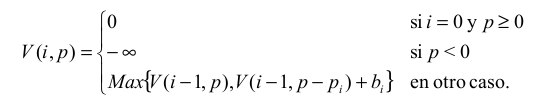
\includegraphics[scale=0.73]{img/mochila01_1}
	\label{contexto:figura5}
\end{figure}